\section{Задание 3: Решение уравнения методом Эйлера}
    \subsection{Постановка задачи}
        Построить графики поведения и фазового решения модели осциллятора Ван
        дер Поля при заданном параметре \(\mu\). Свести уравнение к системе уравнений
        первого порядка. Проанализировать поведение решения системы при разных
        шагах метода Эйлера:

        \begin{align*}
            &y'' - \mu \cdot (1 - y^2)y' + y = 0; \quad \mu = 1.49 \\
            &y(0) = 0.56, ~ y'(0) = 0.22;
        \end{align*}

        Реализацию программы провести на языке <<C++>>.

    \subsection{Решение}
        Сведём уравнение второго порядка к системе уравнений первого порядка:

        \[
            \begin{cases}
                y' = u, \\
                u' - \mu \cdot(1 - y^2)u + y = 0,
            \end{cases}
            \begin{split}
                &y(0) = 0.56, \\
                &u(0) = 0.22, \\
                &\mu = 1.49;
            \end{split}  
        \]

        Рассмотрим следующие шаги: \( 0.1, ~ 0.01, ~ 0.001, ~ 0.0001 \)

        \begin{figure}[H]
            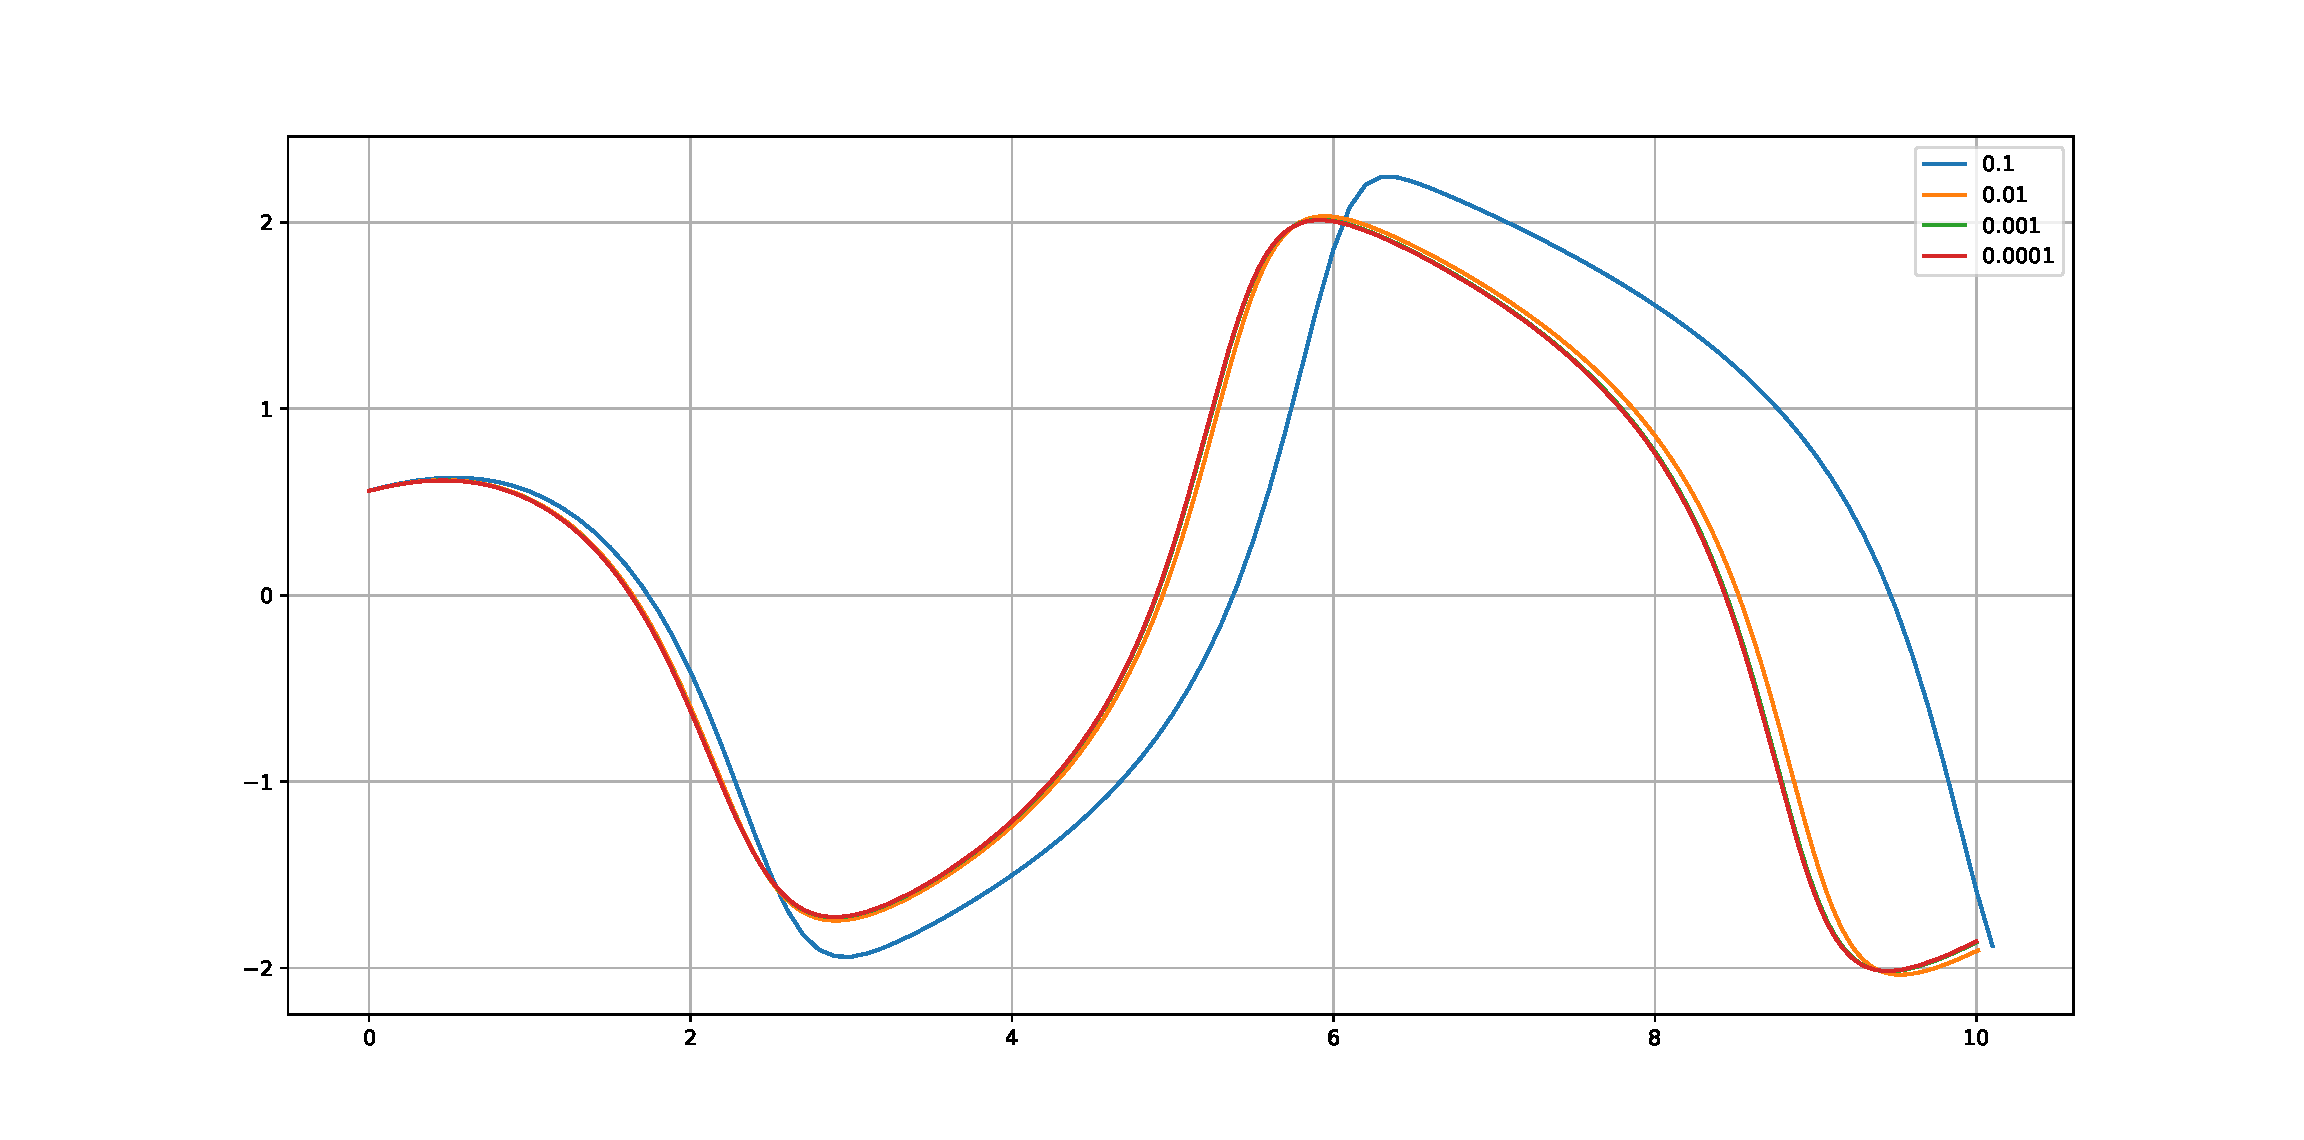
\includegraphics[width=15cm]{pics/3_1.pdf}
            \centering
            \caption{Графики \(y(x)\) при заданных \(h\)}
        \end{figure}

        \begin{figure}[H]
            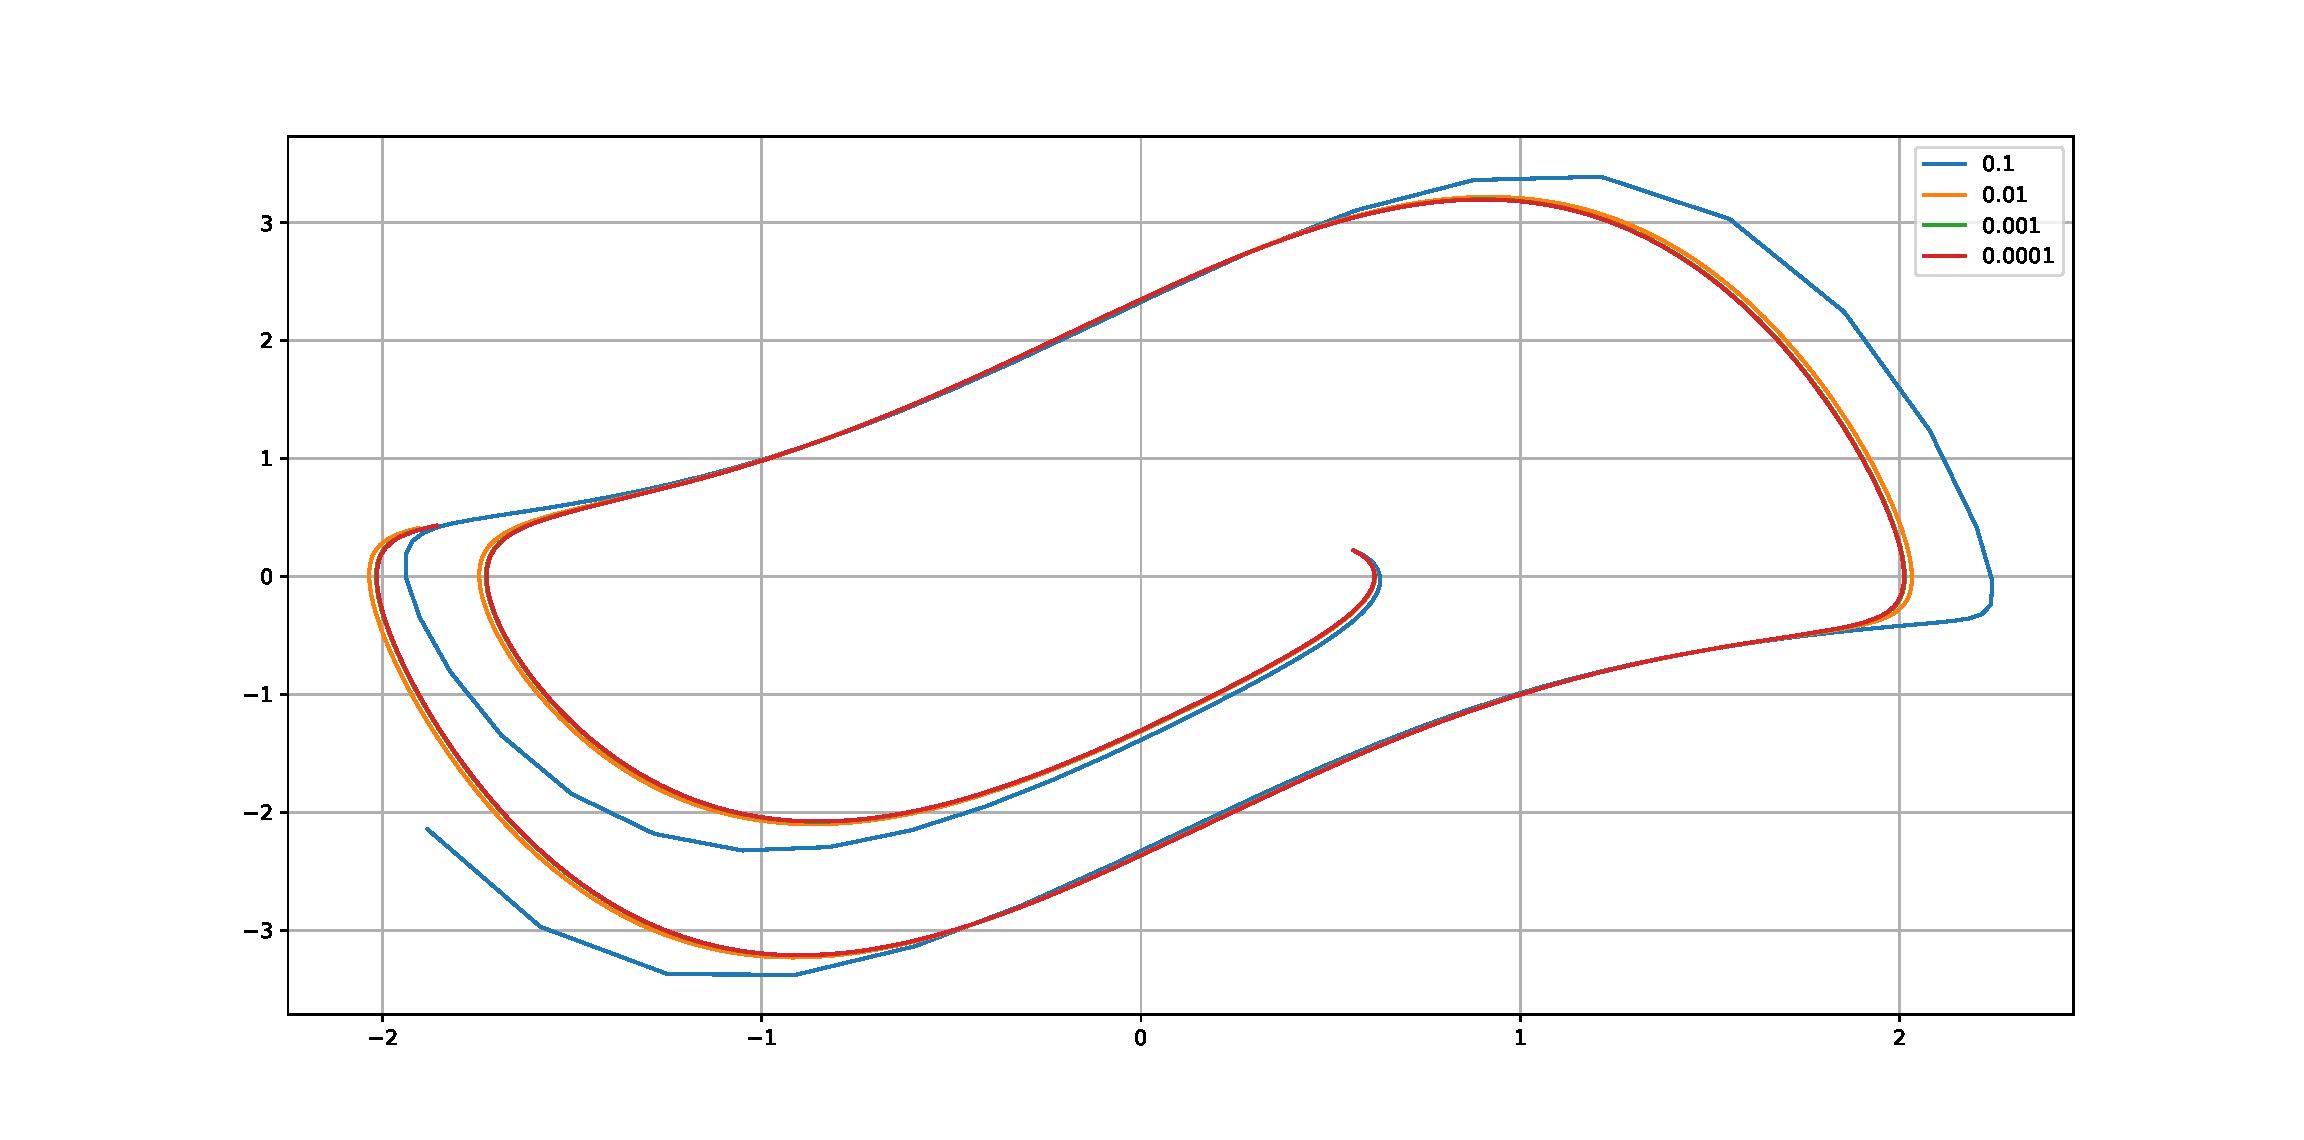
\includegraphics[width=15cm]{pics/3_2.pdf}
            \centering
            \caption{Графики фазового решения при заданных \(h\)}
        \end{figure}

        Исходя из рисунков, можем заключить, что разница между решениями при шагах \(0.001\) и \(0.0001\) не значительна и не видна на графике без должного увеличения. Решение сходится.

        \lstinputlisting[
            language=C++,
            frame=lines,
            caption=Код программы
        ]{src/program.cpp}